\chapter{Conclusion}
\label{chap:conclusion}

The goal of the project was to define, design, and implement a programming
language.  We have accomplished this goal with the creation of \productname{} --
a functional object-oriented programming language in which it is possible to
program board games. In the process we have defined, designed, and implemented
a scanner, a parser, a scope checker, and an interpreter. Furthermore, we have
implemented a simulator which through a game abstraction layer communicates with
the interpreter and in which it is possible to visualise and play
\productname{} games in.

In the analysis chapter (\chapref{chap:analysis}), we have accounted for
different techniques for constructing compilers and interpreters and further
analysed the phases they consist of. In the design chapter
(\chapref{chap:design}) and the implementation chapter
(\chapref{chap:implementation}), we have documented formally and informally how
we have designed, defined, and implemented \productname{}.

In \chapref{chap:requirements} we formulated a list of requirements which
\productname{} and the final solution should be able to fulfil. In
\secref{sec:requirementsevaluation} we evaluated the requirements and the vast
majority of them has been fulfilled. Unfortunately, it was not possible to
implement Chess due to the special rules of the game. The ``En Passant''
and ``Castling'' moves turned out to be more difficult to implement than we
had expected. Although, we still believe that \productname{} provides the
features necessary to get them implemented.

Several well-known board games has already been programmed in \productname{} e.g. Noughts and
Crosses and Connect Four. The games were created in $19$ lines of code and $22$ lines of code respectively (including cosmetic line breaks). We think this clearly shows that it is possible to program board games in \productname{} using only few lines of code.

\section{Discussion}
\label{sec:discussion}

In this section we will discuss what we could have done differently throughout
the project and also discuss future expansion possibilities for \productname{}.

%\subsection{Compile to intermediate language, then translate further}
\label{sec:compiletointermediate}

In this project we decided to implement an interpreter for our programming
language. This decision was made on the basis of our analysis chapter
(\chapref{chap:analysis}) where we could conclude that this would be the optimal
approach for \productname{}, but it is possible to develop a compiler instead. In
this section we will explain what we should have done differently in terms of
the translation method. In \secref{sec:codegenerationandinterpretation} in the
analysis chapter we have analysed and discussed the differences between these
translation methods. Furthermore, in \secref{sec:intermediatelanguage} we
describe what an intermediate language is.

\subsubsection{Where are the differences between an interpreter and a compiler?}

In \secref{sec:compilation} we introduced and explained the phases in the
process of compilation, and with \figref{fig:compileroverview} we visualised
these phases.

The initial phases of a compiler are quite similar to the initial phases of an
interpreter. For instance a compiler must also begin by scanning the source code
followed by parsing the source code to get a stream of tokens and an abstract
syntax tree, respectively. These steps are the same as we have described in
\chapref{chap:implementation}. Furthermore, the step where we check if the
different variables are visible in their respective scopes (scope checking) is
also the same as described in \chapref{chap:implementation}. When the above
mentioned phases have been run then the compiler should compile the code to
machine language or to an intermediate language.

According to \figref{fig:compileroverview} the result of the semantic analyser
would be an intermediate language and then the code generator would generate
machine code which can then be executed. It is of course also possible to compile
directly to machine language. Although, it is not the responsible choice to make 
because it kills opportunities to e.g. optimise the code which would be possible 
with an intermediate language.

\subsubsection{What is the advantage of compiling to an intermediate language?}

When compiling to an intermediate language before compiling to the target
language (often the object code), it is possible to make optimisations on the
intermediate code. This is one advantage of compiling to an intermediate
language and results in more efficient executable code.

Furthermore, one can compile to an intermediate language such as Java bytecode
and the compiled code can be run on every machine that supports Java, which is
very useful because the programmer whom is developing a compiler for the
specific language does not have to construct a compiler for every platform; just
one for Jave bytecode and then translate further to the platform. This way the
programmer must only construct $m+n$ compilers. If one does not compile to an
intermediate language, then the programmer must construct a compiler for each
specific platform, which will be a lengthy process. If you have $m$ compilers
and $n$ platforms, then the programmer must construct $m*n$ compilers to be able
to compile to every platform.  Compiling to an intermediate language and then
further translating is illustrated in \figref{fig:mtimesn}.

\subsection{Compile to intermediate language, then translate further}
\label{sec:compiletointermediate}

In this project we decided to implement an interpreter for our programming
language. This decision was made on the basis of our analysis chapter
(\chapref{chap:analysis}) where we could conclude that this would be the optimal
approach for \productname{}, but it is possible to develop a compiler instead. In
this section we will explain what we should have done differently in terms of
the translation method. In \secref{sec:codegenerationandinterpretation} in the
analysis chapter we have analysed and discussed the differences between these
translation methods. Furthermore, in \secref{sec:intermediatelanguage} we
describe what an intermediate language is.

\subsubsection{Where are the differences between an interpreter and a compiler?}

In \secref{sec:compilation} we introduced and explained the phases in the
process of compilation, and with \figref{fig:compileroverview} we visualised
these phases.

The initial phases of a compiler are quite similar to the initial phases of an
interpreter. For instance a compiler must also begin by scanning the source code
followed by parsing the source code to get a stream of tokens and an abstract
syntax tree, respectively. These steps are the same as we have described in
\chapref{chap:implementation}. Furthermore, the step where we check if the
different variables are visible in their respective scopes (scope checking) is
also the same as described in \chapref{chap:implementation}. When the above
mentioned phases have been run then the compiler should compile the code to
machine language or to an intermediate language.

According to \figref{fig:compileroverview} the result of the semantic analyser
would be an intermediate language and then the code generator would generate
machine code which can then be executed. It is of course also possible to compile
directly to machine language. Although, it is not the responsible choice to make 
because it kills opportunities to e.g. optimise the code which would be possible 
with an intermediate language.

\subsubsection{What is the advantage of compiling to an intermediate language?}

When compiling to an intermediate language before compiling to the target
language (often the object code), it is possible to make optimisations on the
intermediate code. This is one advantage of compiling to an intermediate
language and results in more efficient executable code.

Furthermore, one can compile to an intermediate language such as Java bytecode
and the compiled code can be run on every machine that supports Java, which is
very useful because the programmer whom is developing a compiler for the
specific language does not have to construct a compiler for every platform; just
one for Jave bytecode and then translate further to the platform. This way the
programmer must only construct $m+n$ compilers. If one does not compile to an
intermediate language, then the programmer must construct a compiler for each
specific platform, which will be a lengthy process. If you have $m$ compilers
and $n$ platforms, then the programmer must construct $m*n$ compilers to be able
to compile to every platform.  Compiling to an intermediate language and then
further translating is illustrated in \figref{fig:mtimesn}.

\subsection{Compile to intermediate language, then translate further}
\label{sec:compiletointermediate}

In this project we decided to implement an interpreter for our programming
language. This decision was made on the basis of our analysis chapter
(\chapref{chap:analysis}) where we could conclude that this would be the optimal
approach for \productname{}, but it is possible to develop a compiler instead. In
this section we will explain what we should have done differently in terms of
the translation method. In \secref{sec:codegenerationandinterpretation} in the
analysis chapter we have analysed and discussed the differences between these
translation methods. Furthermore, in \secref{sec:intermediatelanguage} we
describe what an intermediate language is.

\subsubsection{Where are the differences between an interpreter and a compiler?}

In \secref{sec:compilation} we introduced and explained the phases in the
process of compilation, and with \figref{fig:compileroverview} we visualised
these phases.

The initial phases of a compiler are quite similar to the initial phases of an
interpreter. For instance a compiler must also begin by scanning the source code
followed by parsing the source code to get a stream of tokens and an abstract
syntax tree, respectively. These steps are the same as we have described in
\chapref{chap:implementation}. Furthermore, the step where we check if the
different variables are visible in their respective scopes (scope checking) is
also the same as described in \chapref{chap:implementation}. When the above
mentioned phases have been run then the compiler should compile the code to
machine language or to an intermediate language.

According to \figref{fig:compileroverview} the result of the semantic analyser
would be an intermediate language and then the code generator would generate
machine code which can then be executed. It is of course also possible to compile
directly to machine language. Although, it is not the responsible choice to make 
because it kills opportunities to e.g. optimise the code which would be possible 
with an intermediate language.

\subsubsection{What is the advantage of compiling to an intermediate language?}

When compiling to an intermediate language before compiling to the target
language (often the object code), it is possible to make optimisations on the
intermediate code. This is one advantage of compiling to an intermediate
language and results in more efficient executable code.

Furthermore, one can compile to an intermediate language such as Java bytecode
and the compiled code can be run on every machine that supports Java, which is
very useful because the programmer whom is developing a compiler for the
specific language does not have to construct a compiler for every platform; just
one for Jave bytecode and then translate further to the platform. This way the
programmer must only construct $m+n$ compilers. If one does not compile to an
intermediate language, then the programmer must construct a compiler for each
specific platform, which will be a lengthy process. If you have $m$ compilers
and $n$ platforms, then the programmer must construct $m*n$ compilers to be able
to compile to every platform.  Compiling to an intermediate language and then
further translating is illustrated in \figref{fig:mtimesn}.

\input{figures/compiletointermediate}

Now it is alsp possible to optimise the compiled source code before further
translation. So, we can combine these two advantages by developing an optimiser
for the intermediate language. This way all code that has been compiled can be
optimised, which gives better efficiency.


Now it is alsp possible to optimise the compiled source code before further
translation. So, we can combine these two advantages by developing an optimiser
for the intermediate language. This way all code that has been compiled can be
optimised, which gives better efficiency.


Now it is alsp possible to optimise the compiled source code before further
translation. So, we can combine these two advantages by developing an optimiser
for the intermediate language. This way all code that has been compiled can be
optimised, which gives better efficiency.

\subsection{Big integers}
\label{sec:bigintegers}

Our primitive data type to represent numerals with, called Integer, corresponds to Java's primitive data type that goes by the same name. We do not however have an alternative for representing decimal numbers or for representing arbitrary-precision integers if for instance a number is exceeding what's possible to represent with a 32-bit signed two's complement integer. It is imaginable that a programmer of a board game would want to use decimals or very big numbers and therefore implementing this to a later version of \productname{} could be an idea. A possible solution could be a sort of implementation like the bigint and bigdecimal data types of Java. The bigint data type provides analogues to all of Java's primitive integer operators as the primitive data type integer \cite{javabigint} but at the same time it can represent arbitrary-precision integers. That is integers of any size limited only by the memory of the computer. 
\subsection{Artefacts}
\label{sec:artefacts}

In \productname{} games it is not possible to have dice, cards or similar artefacts due to the 
fact that random number generation is not supported. This is a big limitation which decreases the
amount of games possible to program in \productname{} significantly. A game like snake
where a kind of food shows up at random locations on the board or monopoly where a dice decides how
far a player can move and play cards add unforeseen surprises are examples of games which are not possible 
to create. In our game environment described in \secref{sec:gameenvironment} 
many board game related types, constants and functions are implemented. Here it would be natural to also include a
dice type and a card type and related constants like number of eyes on the dice etc.    
\subsection{More actions}
\label{sec:moreactions}

The actions provide everything needed for working with pieces, however when new artifacts are added actions which affects those are needed. An actions to take a card from a deck, an action to play a card, etc. Some artifacts could be generalized: a card could be a \type{Piece} and a deck could be a \type{Square} where the order of multiple pieces is given significance. It is a tradeoff however; generalising will make learning the entire interface easier, but it can make it harder to use


tqweafvkzmsdrx kja sefEWPODGJKL AWE
\subsection{Board types}
\label{sec:boardtypes}

The game environment of \productname{} makes it easy for programmers
to create grid-shaped boards, which is a very basic kind of board
defined by a width and a height filled in with squares. But what if the
programmer wanted to create a circular kind of square or a hexagonal
square? This is currently not possible, but it would be practical in
a future version of \productname{}. A possible solution would be a
graph representation of the board, where the edges represent squares
and transitions represent the border between squares. This would
allow greater expressibility and technically allowing every kind of
imagionable board, even those expanding over time, such as Carcassone.

Patterns, as they are implemented now, only work on grid-shaped boards
because programmers can't define custom \type{Direction} types. To
support all kinds of boards, patterns would have to be able to support
these custom \type{Direction} types. \type{Direction}s would have to be
rewritten so that it'd be possible to define how a certain square is
relative to another (i.e.\ the \type{Direction} would be the label on
an edge going from one square to another).

\subsection{Efficiency of pattern matching}
\label{sec:patternmatchingefficiency}
The design of pattern matching is undoubtedly a strong mechanism for
describing moves, win condition, or any other check that depends on
a particular board layout. Unfortunately, our implementation of the
pattern matching is highly inefficient. Consider the piece placed at
the square D5 in \figref{fig:inefficientpatterns}. The blue piece can
make the moves of a knight from a chess game. This can be specified in
\productname{} with the pattern \texttt{/(n n e|w) | (s s e|w) | (w w
n|s) | (e e n|s) this/}.

\begin{figure}
\centering
\begin{minipage}{.5\textwidth}
  \centering
  \includegraphics[width=.4\linewidth]{pictures/inefficientpatterns}
  \capt{An inefficient implementation.}
  %Pattern matching done on the $8$ green squares will return
  %true, given the moves of a knight and the blue square (D5) as input.
  \label{fig:inefficientpatterns}
\end{minipage}%
\begin{minipage}{.5\textwidth}
  \centering
  \includegraphics[width=.4\linewidth]{pictures/efficientpatterns}
  \capt{An efficient and intuitive implementation.}
  %An efficient and intuitive way to check the moves of a
  %knight piece in a chess game.
  \label{fig:efficientpatterns}
\end{minipage}
\end{figure}

With the current implementation, to find the moves of the piece on D5,
the pattern must be matched on all $64$ squares, given D5 as input.
Those squares for which the pattern matching returns true, are those
squares the piece can move to. In \figref{fig:inefficientpatterns}, only
$8$ of those $64$ checks performed are depicted. For a game of chess
starting with $32$ pieces, the pattern matching is actually done on all
$64$ squares (for all $32$ pieces). If we for simplicity assumed
that each piece had $8$ possible moves, the amount of work related to
pattern checks for the first move in chess can be calculated to be $32
* 64 * 8 = \num{16384}$. Or more generally, $\mathcal{O}(p * n * m *
c)$, where $p = $ the number of pieces, $(n, m) = $ the size of the
gridboard, and $c = $ the complexity of each move. It is easy to see how
inefficient this approach is, so lets now consider a better and more
intuitive approach.

Consider the green piece placed at the square D5 in
\figref{fig:efficientpatterns}. The $8$ arrows show the moves a knight can make.
An easy way to find these squares is simply to start at the knight's square
(D5), move two squares in on of the following directions: north, south, east, or
west, and then one square in an orthogonal direction. This also seems like a
quite efficient approach. This can implemented by modifying the pattern matching
to take a square as input and return a list of squares that satisfy the given
pattern. A pattern for the knight's move could look like \texttt{\%this (n n
e|w) | (s s e|w) | (w w n|s) | (e e n|s)\%}. Notice that the \% $\ldots$
\%-encapsulation is used to distinguish between this modified pattern matching
mechanism from the actual pattern mechanism used in \productname{}, which
encapsulates a pattern between the dots. This modified pattern matching done on
the square D5 would return a list containing the green squares in
\figref{fig:efficientpatterns}, namely the legal moves of a knight on D3.

Compared to the current pattern matching in \productname{}, this approach will
have the complexity $\mathcal{O}(p * c)$. The amount of work related to the
first move of a game of chess would be $32 * 8 = 256$, if we again suppose all
pieces are knights. $256$ is much better than \num{163840} from the previous
example. The complexity here seems to not depend on the actual size of the
gridboard, but this is only true in some cases, e.g.\ when considering the moves
of a knight. If the the moves of a rook are considered, its constant $c$ will
depend on the size of the board for both pattern matching techniques. This is
because a larger board will increase the amount of squares the rook can slide
to. Generally, patterns containing the pattern-value \texttt{*} or \texttt{+}
can have a complexity that depends on the size of the board.

\subsection{Additional functionality with pattern matching}
Many different functionalities could be included in the pattern matching. You
may have noticed the row of black squares in the bottom of the Connect Four game
in \figref{fig:connect4simulated}. These black squares are put there so the
pattern check can allow a piece to be dropped one square north of these squares.
If a pattern keyword \texttt{outofboard} existed that matched a square outside
the board, these squares would not be necessary. A shortcut could also be
considered for specifying patterns of the form \texttt{/(e3) | (w3) | (s3) |
(n3)/}. The \texttt{3} is common, but cannot be used outside parentheses like
\texttt{/(e|w|s|n)3/}, as this means \texttt{/(e|w|s|n) (e|w|s|n) (e|w|s|n)/}.


